%%%%%%%%%%%%%%%%%%%%%%%%%%%%%%%%%%%%%%%%%%%%%%%%%%%%%%%%%%%%%%%%%%%%%%%%%%%%%%%%
%2345678901234567890123456789012345678901234567890123456789012345678901234567890
%        1         2         3         4         5         6         7         8
\documentclass[letterpaper, 10 pt, conference]{ieeeconf}  % Comment this line out
                                                          % if you need a4paper
%\documentclass[a4paper, 10pt, conference]{ieeeconf}      % Use this line for a4

\usepackage{float}
                                                          % paper
% uso paquete bookmark para tener bien los outlines.
\usepackage{bookmark}

% Configuro el idioma.
\usepackage[utf8]{inputenc} % Importante para mantener acentos.
\usepackage[spanish, activeacute]{babel} % Requiere: texlive-lang-spanish. Por primera vez hay que ejecutar: texconfig init> log

% Paquete para poder usar acentos en $$.
\usepackage{mathtools}
%\setmathfont{XITS math}

% Para los diagramas de flujo
\usepackage{tikz}
\usetikzlibrary{positioning}

% colores!
\usepackage{xcolor}

% Elementos del diagrama
\tikzstyle{startstop} = [rectangle, rounded corners, 
minimum width=6em, 
minimum height=2em,
text centered, 
draw=black, 
fill=red!30]

\tikzstyle{io} = [trapezium, 
trapezium stretches=true, % A later addition
trapezium left angle=70, 
trapezium right angle=110, 
minimum width=6em, 
minimum height=2em, text centered, 
draw=black, fill=blue!30]

\tikzstyle{block} = [rectangle, 
minimum width=8em, 
minimum height=3em, 
text centered, 
text width=7.5em, 
draw=black, 
fill=white!30]

\tikzstyle{def} = [rectangle, 
minimum width=14em, 
minimum height=3em, 
text centered, 
text width=12em, 
draw=black, 
fill=purple!30]

\tikzstyle{swap_proccess} = [rectangle, 
minimum width=8em, 
minimum height=2em, 
text centered, 
text width=8em, 
draw=black, 
fill=orange!30]

\tikzstyle{process} = [rectangle, 
minimum width=6em, 
minimum height=2em, 
text centered, 
text width=6em, 
draw=black, 
fill=orange!30]

\tikzstyle{decision} = [diamond, 
minimum width=6em, 
minimum height=6em, 
text centered, 
draw=black, 
fill=green!30]
\tikzstyle{arrow} = [thick,->,>=stealth]

\usepackage{siunitx}

% package to get \url
\usepackage{hyperref}
\hypersetup{
  colorlinks=true,
  linkcolor=magenta,
  filecolor=magenta,
  citecolor=magenta,      
  urlcolor=magenta,
}

% Graficos electrónicos
\usepackage{circuitikz}

\IEEEoverridecommandlockouts                              % This command is only
                                                          % needed if you want to
                                                          % use the \thanks command
\overrideIEEEmargins
% See the \addtolength command later in the file to balance the column lengths
% on the last page of the document

\usepackage{graphicx}
\usepackage{graphics}

% styling for matlab/octave code.
\usepackage{matlab-prettifier}
% Configuracion, con esto puede agregar ñ.
\lstset{
  literate={ñ}{{\~n}}1
}

\usepackage{listings}

% The following packages can be found on http:\\www.ctan.org
%\usepackage{graphics} % for pdf, bitmapped graphics files
%\usepackage{epsfig} % for postscript graphics files
%\usepackage{mathptmx} % assumes new font selection scheme installed
%\usepackage{times} % assumes new font selection scheme installed
\usepackage{amsmath} % assumes amsmath package installed
%\usepackage{amssymb}  % assumes amsmath package installed

\title{\LARGE \bf Laboratorio N° 1}

\author{
  Tom\'as Vidal\\
  {\it Control Automático II}\\
  {\it Facultad de Ingenier\'ia, UNLP, La Plata, Argentina.}\\
  {\it 6 de Mayo, 2024.}
}                                            % <-this % stops a space


% comienzo

% INTRO


% Figura
\newcommand{\image}[2] {
  \begin{figure}[H]
    \centering
    \includegraphics[width=0.43\textwidth]{./#1.png}
    \caption{#2}
    \label{fig:#1}
  \end{figure}
}

% Codigo
% \begin{lstlisting}[style=Matlab-editor]
% % el código va aca
% dispc("HELLO WORLD");
% \end{lstlisting}

\begin{document}
\maketitle
\thispagestyle{empty}
\pagestyle{empty}

\section{Diagrama Eléctrico Esquemático}
\begin{figure}[H]
  \centering
  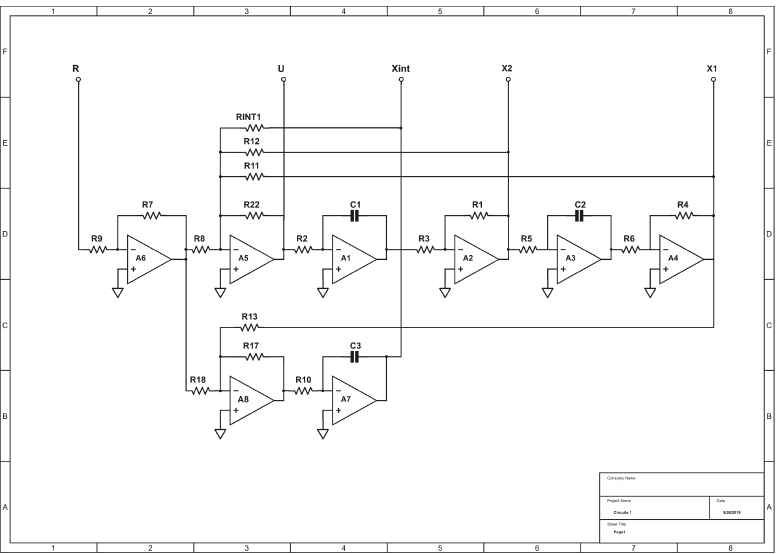
\includegraphics[width=0.43\textwidth]{./Imagenes/DiagElecEsquematico.png}
  \caption{Diagrama eléctrico esquemático del circuito provisto}
  \label{fig:diag_elect_esq}
\end{figure}

En el diagrama \ref{fig:diag_elect_esq} se pueden identificar diferentes bloques que cumplen distintas funciones. Estos están identificados en el diagrama \ref{fig:diag_elec_esq_etapas}, y sus funciones se detallan a continuación:
\begin{itemize}
  \item \textbf{Inversor:} crea un desfase de \ang{180} a la salida respecto de la entrada (\textit{color rojo}).
  \item \textbf{Sumador inversor:} suma todas las señales en la entrada y luego desfasa el resultado en \ang{180} (\textit{color azul}).
  \item \textbf{Integrador inversor:} integra la señal de entrada y la desfasa en \ang{180}  (\textit{color verde}).
\end{itemize}
\begin{figure}[H]
  \centering
  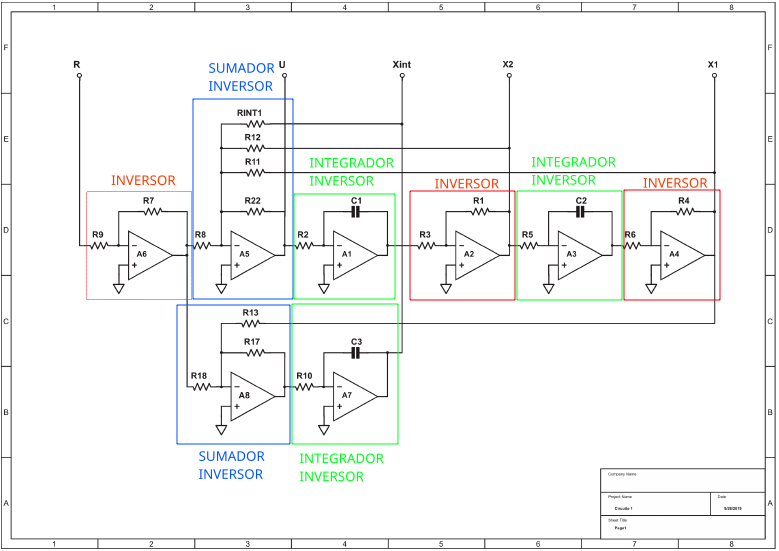
\includegraphics[width=0.43\textwidth]{./Imagenes/DiagElecEsqEtapasIdent.png}
  \caption{Se identifican las etapas funcionales del diagrama \ref{fig:diag_elect_esq}}
  \label{fig:diag_elec_esq_etapas}
\end{figure}

Además se pueden identificar tres bloques principales que están compuestos por los previos. Los mismos se pueden identificar en \ref{fig:diag_elec_esq_bloques_principales} y corresponden a:
\begin{itemize}
  \item \textbf{S:} Bloque de control.
  \item \textbf{H:} Bloque de lo que simula ser el sistema o la computadora analógica.
  \item \textbf{I:} Bloque de compensación o de corrección de errores.
\end{itemize}

\begin{figure}[H]
  \centering
  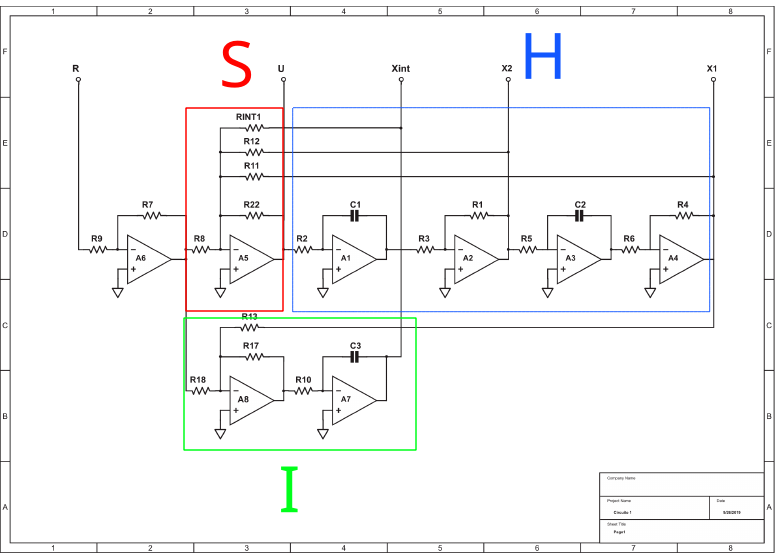
\includegraphics[width=0.43\textwidth]{./Imagenes/DiagElecEsquematicoBloquesPrincipales.png}
  \caption{Bloques principales del diagrama \ref{fig:diag_elect_esq}}
  \label{fig:diag_elec_esq_bloques_principales}
\end{figure}

\subsection{Transferencias de los bloques}

\begin{itemize}
  \item Sistema
    \begin{equation} \label{eq:trans_H}
      \begin{cases}
        X_2 = \frac{U}{C_1R_2S}                     \\
        X_1 = \frac{U}{(C_1R_2S)(C_2R_5S)}          \\
        \frac{X_1}{U} = \frac{1}{(C_1R_2S)(C_2R_5S)} \\
        H = \frac{X_1}{U} = \frac{H_0}{s^2}           \\
        H_0 = \frac{1}{C_1R_2C_2R_5}
      \end{cases}
    \end{equation}
  \item Control
    \begin{equation}
      \begin{cases}
        R = U - a_ix_{int} - a_2x_2 - a_1x_1             \\
        a_i = \frac{R_{22}}{R_{int}}                     \\
        a_1 = \frac{R_{22}}{R_{12}}                     \\
        a_i = \frac{R_{22}}{R_{11}}
      \end{cases}
    \end{equation}
  \item Compensador
    \begin{equation}
      X_{int} = \frac{-(R-X_1)}{R_{10}C_3S}
    \end{equation}
\end{itemize}

\subsection{Controlabilidad y Observabilidad}
Para analizar la controlabilidad primero se determinaron las matrices \textbf{A} y \textbf{B} del sistema \textbf{H}, y luego se llevó a \textbf{A} a su forma canónica controlable:
\begin{equation} \label{mat:a_de_h_cano_contr}
  A =
  \begin{bmatrix}
    0 & 1\\
    0 & 0
  \end{bmatrix}
\end{equation} 

\begin{equation} \label{mat:b_de_h_cano_contr}
  B =
  \begin{bmatrix}
    0\\
    1
  \end{bmatrix}
\end{equation} 

\begin{equation} \label{mat:c_de_h_cano_contr}
  C =
  \begin{bmatrix}
    H_0 & 0
  \end{bmatrix}
\end{equation} 

Como se puede observar en \ref{mat:a_de_h_cano_contr}, el sistema tiene un polo doble en el origen, debido a que los autovalores de la misma son $\lambda^{2}=0$, que concuerda con lo que se observa en las Transferencias obtenidas previamente en \ref{eq:trans_H}.

Para analizar la observabilidad se llevó a su forma canónica observable y como el rango de la matriz de observabilidad es de rango se concluye que es observable.
\begin{equation} \label{mat:observabilidad}
  O =
  \begin{bmatrix}
    H_0 & 0\\
    0   & H_0\\
    0   & 0\\
    0   & H_0
  \end{bmatrix}
\end{equation} 

\section{Posible análisis experimental}
Para poder analizar que la respuesta del sistema corresponda con lo teórico, se podría llevar el sistema a un estado de oscilación, ya que su condición de establidad es crítica va a tener una respuesta oscilatoria correspondiente a la de un sistema de orden 2 cuando se efectúe en la realidad, entonces una vez en este estado oscilatorio se podría medir la constante de tiempo y así determinar los parámetros correspondientes.

\end{document}
